\documentclass[a4paper]{article}
\usepackage{lipsum}
\usepackage{url}
\usepackage{graphicx}
\usepackage{listings}
\lstset{language=Python}
\usepackage[margin=2cm]{geometry}
\usepackage{indentfirst}
\usepackage{xcolor}
\usepackage{lmodern}
\usepackage{enumitem}
\usepackage{multicol}
\renewcommand{\familydefault}{\sfdefault}
\graphicspath{ {images/} }

\begin{document}

% TODO: Anything else needed for titlepage
% TODO: Adjust the spacing between bullet point sections
\begin{titlepage}
	\newcommand{\HRule}{\rule{\linewidth}{0.5mm}}
	\center{}

    %Headings
	\LARGE{University of Nottingham}\\[1.5cm]
	\Large{Computer Science with Artificial Intelligence MSci}\\[0.5cm]
	\large{G54IRP/COMP4027 --- Individual Research Project}\\[0.5cm]

    %Title
	\HRule{}\\[0.4cm]
	{\huge\bfseries AI for General Video Game Playing}\\[0.4cm]
	\HRule{}\\[1.5cm]

    %Authors
	\begin{minipage}{0.4\textwidth}
		\begin{flushleft}
			\large
			\textit{Author}\\
			Benjamin Charlton\\
            psybc3@nottingham.ac.uk\\
            4262648
		\end{flushleft}
	\end{minipage}
    \begin{minipage}{0.4\textwidth}
		\begin{flushright}
			\large
			\textit{Supervisor}\\
			Dr.\@ Ender \"Ozcan\\
            Ender.Ozcan@nottingham.ac.uk
		\end{flushright}
	\end{minipage}

    %Date
	\vfill\vfill\vfill
	{\large7\textsuperscript{th} December 2017}
	\vfill

\end{titlepage}

%Contents Page
\pagenumbering{roman}
\tableofcontents
\pagebreak

\pagenumbering{arabic}
\section{Introduction}
\subsection{Introduction}
\begin{itemize}
    \item Popularity of Video Games
    \item Variety of Video games being played
    \item Video Games as a testing ground for AI
\end{itemize}
\subsection{Planning VS learning}
\begin{itemize}
    \item As the title says, just to get some definitions out of the way
\end{itemize}
\subsection{Motivation}
\begin{itemize}
    \item Individual desire to get better at deep reinforcement learning
    \item Learning more Methods
    \item Applying Methods
    \item Learning to use more robust and real world frameworks for DRL
    \item
    \item Seeing the state of the art in DRL and AI game playing
\end{itemize}
\subsection{Aims and Objectives}
\begin{itemize}
    \item Look at the project plan aims and objectives
    \item
    \item Discuss how we will be using OpenAI Baselines to test
    Like the GVGAI Gym paper but applying it in a general setting.
    \item Would like to get it working like in the competition (3 games 3 levels training, same games 2 levels validation).
    \item Maybe run it on a larger sample of games in the same way.
    \item Train on all levels of several games and see if it can just pick up an unseen game.
\end{itemize}

\section{Related Work}
\subsection{AI and Game Playing}
\begin{itemize}
    \item ALE --- Learning works for games
    \item Conclusion for this section
\end{itemize}

\subsubsection{Early Artificial Intelligence}
%TODO: Maybe extend / re sort this section
The history of AI game playing begins near the start of artificial intelligence as a field, in the 1950s.
Strachey created a draughts player for one of the first general computing machines (Manchester Ferranti Mark I) which by  1952 could ``play a complete game of draughts at a reasonable speed''\cite{BreifHistoryComputing}.
Prinz wrote a simplified chess player for the Manchester Machine as well which could solve the mate-in-two problem.
This meant that if there was a checkmate solution in 2 turns it could successfully find it\cite{BreifHistoryComputing}.
Prinz simply used an exhaustive search technique to find the correct moves, and even though computing power was limited at the time it was clear that this wouldn't scale to full games.
This lead to Turning starting to program `Turbochamp' a chess program that would be able to play a full game of chess using heuristics\cite{BreifHistoryComputing}
\par
These simple games were made before the term artificial intelligence was being used even in an academic setting showing how natural AI and game playing go together.

\subsubsection{Deep Blue --- Chess}
Chess was an early and significant example in the history of AI game playing.
In 1997 IBM managed to beat the reigning world champion, Garry Kasparov, using their custom developed machine, Deep Blue\cite{deepBlue}.
This was significant as, at the time, creating a winning chess AI was seen to be the next big milestone at the time in AI\@.
\par
To achieve this Deep Blue used a combination of techniques with the main underlying AI technique being a search method.
As Chess is a deterministic game and both players have complete information of the board state it was possible for Deep Blue to generate future board states.
With this forward model its possible to generate a search tree of possible moves and their resulting game states
The tree was efficiently generated by a combination of a massively parallel architecture over 30 nodes and the fact that each node has special purpose chess chips, generating around 6--8 moves ahead on average.
Alpha-beta pruning was used in a MinMax algorithm to help efficiently search the tree while using the custom hardware to evaluate each node quickly.
\par
IBM had proven that search methods could achieve strong results against human opponents but this was mostly due to brute force computing power and a heavy reliance on expert knowledge.
The expert knowledge came from other grandmasters and was used in the form of an opening/closing move database and the special purpose hardware to evaluate board states.
While higher computing power will always benefit AI techniques, later techniques have been developed to reduce the need of expert knowledge and to make more efficient use of hardware available.

\subsubsection{AlphaGo --- Go}
Although Deep Blue had proven that AI systems could beat an expert in games, the methods used wouldn't scale to more complex games such as Go, new methods would be needed to tackle more complex games and to further the field of AI\@.
Go was set as the next milestone in AI game playing by the community as it proved vastly more complex than chess while still having few rules and a simple goal, like chess.
To compare the difficulty between the 2 games, chess uses a 8\(\times \)8 board while Go uses a 19\(\times \)19 board.
What is a better indicator of the AI performance is the branching factor of the games for each move, as this more accurately shows how large the search tree grows for each possible move.
On average, Chess has a branching factor of 35 and Go has a branching factor of 250\cite{BranchingFactor}.
In 2016 DeepMind reached this milestone with AlphaGo claiming its victory against a 9th dan professional Go player, Lee Sedol, in March 2016\cite{alphaGo}.
\par
This achievement was accomplished with a combination of Monte Carlo Tree Search (MCTS) and 2 Deep Neural Networks trained with reinforcement learning, one was a value network to assess the board predicting the winner and the other a policy network to predict which move would be played next by an expert.
By augmenting MCTS with the policy network, the problem of the large branching factor was greatly reduced, the value network made the addition that it was quicker and more accurate at determining who would win than conventional methods and didn't require an ending game state to be reached.
Initially these networks were trained on a large number of human played games as a labeled dataset, after this `boot strapping' phase they were trained through instance of self play.
\par
Between October 2015 and AlphaGo's retirement in May 2017 there were 3 significant versions of the AI system.
AlphaGo Fan was named after its opponent Fan Hui a European 2nd dan professional Go player, where it won 5--0 being the first ever computer to beat a human professional at Go without a handicap.
AlphaGo Lee was named after its opponent Lee Sedol a South Korean 9th dan professional Go player, in this match AlphaGo won 4--1 and was seen as an AI system successfully beating a Go champion at their own game.
AlphaGo Master was the final version of the system and was named after the online account it played on for 60 Games against human opponents, it managed to win all 60 games and was finally revealed to have been a computer system to the Go community.
It finally retired at the Future of Go summit where it played a further few games beating another champion Ke Jie and a human team of 5 Go professionals.
After the summit it was clear that AlphaGo was a champion of the game and as a gift to the Go community they presented a series of 50 games for people to analyse.

\subsubsection{AlphaGo Zero --- Go}
After retiring AlphaGo Deep Mind was already working on a successor that would seek to fix some of the downsides of the AlphaGo system.
They sought to create a system that could play `tabula rasa' (latin for from a blank slate) requiring human expert decisions to learn from as they say that `Expert data sets are often expensive, unreliable or simply unavailable'\cite{alphaGoZero}.
The problem came from the initial supervised learning stage of AlphaGo's development, as it required millions of human expert games with the correct outcomes to initially learn from before it began using reinforcement learning and self play to hone its skills.
\par
There are many issues often associated with using supervised learning, 3 of the main issues were brought up when describing the expense, reliability and the availability of these datasets.
While AlphaGo had proven that there was suitable enough data for learning the game of Go, a motivating factor for the team was showing that this wasn't needed and hopefully find a method that could then later be adapted to other problems with these issues.
Another issue was a notion of a skill ceiling, as such to say that the system can only learn to be as good as the data provided to it an idea that is also seen in human learning where a student can only be as intelligent as their teachers.
This was to say that if a system learnt from human experts then it would only slightly build upon the expert knowledge where as their could potentially be ideas unconsidered by humans that could lead to a stronger system.
AlphaGo had shown evidence of this when it played a so-called `divine move' against Lee Sedol indicating there was more potential for innovation in strategy even in an ancient classic game like Go.
Furthermore by also not having a reliance on human expert knowledge an AI system could be developed to complete task where there is limited or no expert knowledge to help guide it.
\par
AlphaGo Zero differs in 4 key ways to its predecessor AlphaGo:
\begin{itemize}
    \item It trained by selfplay reinforcement learning exclusively, starting with random play.
    \item It only used the 19x19 board with the stone colours as input.
    \item It used a single neural network rather than 2.
    \item A simpler tree search was used not requiring a Monte Carlo rollouts
\end{itemize}
By using this form of selfplay it means that AlphaGo Zero gradually improved after every game, but it also allowed for it to have an equally strong opponent at every step of the learning process.
This results in games which much more can be learnt from as it is hard to learn from a system if you are always winning or losing.
\par
The single neural network was designed to take in the raw current board state and output a prediction value of the chance to win and a vector of move probabilities.
This was compared with the true winner of the game from the self play and the search tree probabilities.
The comparison formed the loss function of the neural network and was updated via gradient descent.
\par
The network is used by the search algorithm by selecting the likely moves to make and searching a few moves forward, using the networks winner prediction to select a strong move to make where it has the greatest chance of winning.
\par
Ultimately when tested against different versions of AlphaGo, AlphaGo Zero won with conclusive results.
Winning 100--0 against AlphaGo Lee and 89--11 against AlphaGo Master.
They also gave a rating to a version of AlphaGo Zero that just used the neural network, selecting the move it thought would have the highest probability of winning without using a tree to look ahead.
This neural network only system didn't out perform any version of AlphaGo but it came about 3\% lower than AlphaGo Fan and was 50\% stronger than any other Go AI tested.
\par
Although AlphaGo Zero was intended to work without any human domain knowledge, some was used to help the training process.
In particular the game of Go is invariant under rotation, reflection and colour transposition allowing for the same board to be used for training multiple times, vastly increasing the amount of training data generated for the neural network.
The MCTS that was used to help train the network (not play) was given perfect knowledge of the rules of Go as well.

\subsubsection{OpenAI Five --- DotA 2}
While board games have found great success in the AI game playing space, video games haven't seen as much popularity due to complexity of both the games and integrating the AI system and the game together.
\par
An attempt to combine AI and game playing was the OpenAI team in the game DotA 2.
DotA 2 is typically a 5v5 team game with a cast of over 100 characters with multiple abilities and items they can use.
It is played from a top down perspective with each game taking place on the same map every time.
As of the time of writing the have been over 10 million unique players in the last month\cite{DotA2}
\par
To help with the complexity of the problem the initial challenge that was tackled was a simpler version of DotA 2 namely 1v1 matches.
Even though this is a scaled down version of the whole game; Elon Musk, backer of this initiative, said that this is `Vastly more complex than traditional board games like chess \& Go'\cite{OpenAI}.
On top of being scaling down the game the team further limited the games to only be played with a single character for both players so that the bot didn't have to learn several character although most 1v1 DotA tournaments use this rule.
The system was first shown off during the 2017 International, the largest DotA 2 tournament featuring a prize pool of nearly \$25 million (USD), to a live audience of DotA 2 fans.
It played a best of 3 1v1 match against one of the best DotA 2 players in history, Dendi, where the AI convincingly won game 1 and Dendi conceded the second game when he realised he was unable to win.
\par
To achieve this astonishing result against not only Dendi but several other professional DotA 2 players, a LSTM Neural Network was trained using selfplay reinforcement learning.
By using the games API it had access to the game state rather than just using the screen input, although this could be seen as an advantage to the AI no information can be got from the API that wouldn't be available to the player looking at the screen.
This allowed for the AI to very easily take input from the game into its neural network and the output to be a valid actions.
\par
The system has been extended into one know as `OpenAI Five', named after the 5 individual neural networks used to create a 5 player team of DotA 2 AIs\cite{OpenAIFive}.
Each of the 5 neural networks are identical but train to play a different character.
These neural networks trained with no human data like AlphaGo Zero, once again proving that contrary to popular belief this isn't needed to create powerful systems.
Unlike a human team the OpenAI Five didn't have a communication channel between the different AIs but were trained to work together and not maximise their reward at the detriment of the teams.
This is a massive step forward towards playing a full game of DotA 2 but there are still some limitations of the system, such as it can only play the same 5 characters and the opposing team also needs to use the same 5 characters.
Certain mechanics of the game were also not implemented into the neural network structure so they can't be used by either the OpenAI Five or its opponents.
Since the initial report some of these restrictions have been lifted and the OpenAI Five can play and play against 18 characters vs 5 originally.
\par
So far OpenAI Five has been performing well against amateur to semi-professional teams, even going as far as beating a team composed of players in the top 99.95th percentile of DotA 2 players.
During the International 8 in August 2018, OpenAI Five played against a top professional team who trained together with most of the restrictions lifted.
This resulted in a game that most people believed to be much closer to the full DotA 2 game.
Unfortunately OpenAI Five lost these games but the team said `Remarkably, the games were exciting and close'\cite{OpenAIInternational}.
The team behind OpenAI Five, OpenAI, believes that the rule changes weren't why they lost, but they need to move forward reducing the number of scripted logic in the system, removing bugs and letting the system train for longer.

\subsubsection{Atari}
\begin{itemize}
    \item No Idea about this would have to do some significant research into the topic to write it up.
\end{itemize}

\subsubsection{AlphaZero}
\begin{itemize}
    \item No Idea about this would have to do some significant research into the topic to write it up.
\end{itemize}

\subsubsection{Conclusions}
\begin{itemize}
    \item Deep Blue proves that games can effectively use forward planning to beat human experts, early techniques require a lot of power so intelligent methods are needed to speed up results/improve search depth
    \item AlphaGo Fan, Lee and Master show planning is still effective but by using more advanced techniques we can generate search trees better (ANNs).
    Also shows how learning can benefit AI techniques and boost the powerful planning techniques.
    \item AlphaGo Zero shows how learning doesn't need to require expert knowledge and can just learn from lots of experience in the environment
    \item AlphaZero shows how more generic systems can still perform well allowing for techniques that could be transplanted into many environments and still perform well.
    Also showing that although dedicated hardware was used no purpose built hardware or software was used to exploit features of the games unlike previous versions or Deep Blue.
    \item AlphaGO Zero using only the network doesn't achieve state of the art performance but comes close and doesn't rely on a look ahead style search tree.
\end{itemize}


\subsection{GVGAI and VGDL}
\begin{itemize}
    \item TODO Make some notes up here
\end{itemize}
\subsection{OPEN AI GYM and GVGAI GYM}
\begin{itemize}
    \item What is OPEN AI GYM
    \item Why is OPEN AI GYM helpful for RL
    \item GVGAI GYM
    \item Initial results from GVG AI GYM paper
    \item Maybe some more here
\end{itemize}\cite{GVGAIGYM}

\subsection{Subsection to end all subsections}
\begin{itemize}
    \item Maybe something about the open AI baselines
    \item Depends what technique I would be using but I should look into that
    \item Where does reinforcement learning come into this bad buoy
\end{itemize}

\section{Progress}
In this section the progress made up until the writing of this report will be discussed alongside any modifications that were made to the work plan, changes to future plans based upon the work so far will be discussed in the next section.
\subsection{Modifications to the Work Plan}
Some tasks have been modified to due to various factors, such as them taking longer than expected or new additions to help make easier progress.
An up to date version of the work plan has been included in the appendix showing an accurate depiction of what tasks were completed over the previous term, with changes highlighted in a bold box.
This can be seen in TODO INSERT SECTION 5.3.1.
Following is a list of modifications that have been made and the reasons behind these changes.
\begin{description}
\setlength{\itemsep}{0pt}
\setlength{\parskip}{0pt}
\item [\large{Documentation}]
\item [D4--Interim Report Outline Sections]
This was pushed back a week to accommodate for the addition of task C5.
\item [D5--Interim Report Related Work]
Extended the writing of the related work section due to the larger amount of research done that was needed to be talked about.
This is due to the project taking a large research focus for the first term than initially expected and compared to previous projects.
\item [D6--Interim Report Draft]
This was pushed back a week to accommodate for the addition of task C5.
\end{description}

\begin{description}
\setlength{\itemsep}{0pt}
\setlength{\parskip}{0pt}
\item [\large{Research}]
\item [R5--Other Related Works]
This was extended from 2 to 4 weeks to accommodate for the addition of task C5 and to allow for more papers to be researched after seeing a wide variety of relevant and informative papers.
\end{description}

\begin{description}
\setlength{\itemsep}{0pt}
\setlength{\parskip}{0pt}
\item [\large{Development}]
\item [S3--Run available previous agents]
As there was no previous agents available using the latest framework, previous agents couldn't be ran in the same framework that the project was being developed in.
Rather than spending time installing a previously used framework it was decided that it would be simpler and more effective to just use the results in the research articles instead of running the agents to compare them.
\item [S5--Develop Keyboard Controller]
While trying to debug some issues with the framework it became clear that it would be easier to test if the GVGAI games could be directly controlled by a user.
For this reason a keyboard controller was made to allow for user controlled games.
\end{description}

\begin{description}
\setlength{\itemsep}{0pt}
\setlength{\parskip}{0pt}
\item [\large{Miscellaneous}]
\item [M4--Plan 2\textsuperscript{nd} Stage of the Project]
This part was brought forward a week to align with the writing of this report.
This allows for this report to contain a plan for the second stage and moving it forward doesn't massively clash with other aspects of the project.
\end{description}

\begin{description}
\setlength{\itemsep}{0pt}
\setlength{\parskip}{0pt}
\item [\large{Other Commitments}]
\item [C5--GameSoc Varsity \& HackNotts]
This was added as 2 large university society events that I was volunteering at were taking place during this time.
This meant that project work was postponed to allow concentration on the successful running of these events
\end{description}

\subsection{Current Achievements}
In this part, any significant progress will be described outlining what was done and how it has helped the project move forwards.

\subsubsection{Learning the GVGAI, OpenAI Gym and GVGAI Gym Frameworks}
A lot of time has been spent learning various frameworks that are used within the GVGAI competition and will be used in this project.
By using these frameworks significant amounts of work that would be required to create games or successfully interface with previous ones has been reduced.
Despite this time has still been spent on learning hope the frameworks operate to use them effectively.
Some of the following achievements put the knowledge gained from learning these frameworks to use in creating useful tools.

\subsubsection{Action Space Analysis}
Due to how recent the GVGAI Gym framework is, some elements of the how the games worked were unclear.
One such element was the action space of the agents which corresponds to the inputs for the games.
To answer any questions, a small script was written to analyse the action space of all the environments.
\par
The following was discovered:
\begin{description}
\setlength{\itemsep}{0pt}
\setlength{\parskip}{0pt}
\item [Total number of actions]
Across all the games the same 6 actions were used, listed below with their typical meanings.
\begin{multicols}{2}
    \begin{itemize}
        \item ACTION\_NIL --- Make no action
        \item ACTION\_USE --- Interact in game
        \item ACTION\_LEFT --- Move the character left
        \item ACTION\_RIGHT --- Move the character right
        \item ACTION\_DOWN --- Move the character down
        \item ACTION\_UP --- Move the character up
    \end{itemize}
\end{multicols}
\item [Not all games used all actions]
While every game had a ACTION\_NIL action, some games didn't use all of the other actions.
This means that for some games the action space is smaller than others and this would have to be taken into account when making an AI to play all the games, as trying to use an incorrect action could cause unpredictable behaviour in a AI system but will also result in disqualification in the GVGAI competition.
Simple solutions to this problem could be passing an ACTION\_NIL if the AI tries to use an action that isn't available in the current game, or to selected the next best choice of action as given by the AI\@.
\item [The Actions weren't numbered the same]
The action descriptions have been used so far to give an idea of what each action does, the labels are from the old GVGAI framework where these where used as an enum to describe each action.
In a discrete OpenAI Gym environment, which the current GVGAI Gym is, the action space is represented as a set of numbers corresponding to the actions order.
While the actions are always ordered the same way (ACTION\_NIL will always be first and ACTION\_UP last) if an action is not used in that game and therefore not present it will mess up the numbering.
This means care needs to be taken in games that don't use all the actions so that the correct action is given to the environment.
\end{description}

\subsubsection{Keyboard Controller}
It became apparent that a way for a human to interact with the various environments would prove useful for development and debugging.
The majority of the code for this was reused from the OpenAI Gym keyboard controller\cite{OpenAIGym}, which can be found in their GitHub repository.
\par
The modifications made allowed for relevant logging to the console, better controls, displaying the controls to the user at the start, and setting a game tick rate/ frame rate to be the same as the GVGAI competition.
The WASD keys were bound to movement and use on the J key, this is closer to what typical games would use making it easier to pick up for people used to playing on a keyboard already.
The frame rate is set rather low for games at 25fps but it can be changed in the program, 25fps is used as that is both smooth enough and gives the same decision and reaction time as the AI system will get.
Although this does make it much simpler for any human player to succeed in trickier parts of a game, even making frame perfect timing relatively easy for most humans.
\par
Although originally intended to aid development this tool could be used to compare an AI system against human skill of varying levels.

\subsubsection{Random Agent}
To help understand the framework and to generate a point of comparison, a simple random agent was made.
It works by knowing the the possible actions across all games and choosing one at random, if that action isn't in the list of actions in the game currently being played it will then reselect an action.
This is a simple solution to get around the fact that not all actions are used in all games.
It samples all actions uniformly with no bias to a particular action.
\par
The random agent is wrapped in a program that allows it to be ran in any of the environments.
There are also settings to allow the choice of rendering the game screen to the user so the agent actions can easily be shown, as well as a setting to modify the number of game ticks that the game will be ran for.

\subsubsection{Testing Agent in multiple Environments}
Another help tooler created was one that could run a given agent in multiple of the environments to test how well it performs in the environments.
It is currently set up to run the random agent in all of the environments (bar a few that have been crashing).
It also runs the agent in each environment a few times so that random variation (in the game or agent) can be accounted for.
\par
As there are many environments to run the agent in, this tool makes effective use of multiprocessing allowing a significant speed up in the generating of data.
For each run in an environment the following data is collected:
\begin{multicols}{2}
    \begin{itemize}
        \item Game --- The game being played
        \item Level --- The level of the game
        \item Version --- The game version
        \item Score --- The final score at the game end
        \item Winner --- Wether the agent won
        \item Game Tick --- The game tick when the game ended
    \end{itemize}
\end{multicols}
These results are stored as a json object and parsed together with all the other results to create a list of all of the results.
As the list is in a json format it can be easily analysed at a later date, or combined with other runs to create a larger dataset.
\par
\begin{itemize}
    \item Do I analyse and put the random agent results in here?
\end{itemize}
\par
This tool will become incredibly useful when testing an agents performance across a variety of games due to its quick running time.
It is also simple to test multiple agents using this tool so that they can be compared to each other.
As the tool returns the raw data it can be analysed in whatever way suits the current scenario, such as even though the random agent has been run in all of the environments we can easily compare it to another agent in a handful of those environments by simply selecting the correct data points from the random agent results for comparison.

\subsection{Reflections on Current Progress}
On the whole the work plan has been stuck to, allowing for easy knowledge of where the project is up to at any time and clear progress to be made.
The minor changes to the work plan have on the whole been made to aid with management of large tasks and other commitments.
Although a few tasks were delayed the major milestones have been stuck to so far, namely finishing of development tasks and writing the interim report.
\par
A personal issue with progress was the lack of deliverables with the major research section of the project.
This section took up over 50\% of the time spent on the project so far.
This time was spent by self guided study, finding and reading relevant works to the project.
With the lack of deliverables it was hard to judge if enough research had been completed, or if a wide enough scope was researched.
Another issue with the research was time spent researching and understanding older frameworks which bare little to no relevance on the project moving forward.
Spending hours researching a topic to only realise it is not what you thought it was on initially led to some frustration.
\par
To aid with project management and accountability meetings have taken place, with a regular slot set aside to allow for agile meetings.
These have often discussed upcoming tasks in relation to the work plan and what work has taken place.
For each meeting a short set of minutes was created and emailed to attendees, allowing for all parties to know what was discussed and what was to happen before the next meeting.
All of the minutes can be found in the appendix, section TODO INSERT SECTION 5.2.

\section{Next Steps}
This section will outline the next steps in the project as directed by the research done into what methods are effective.
All of these steps are also outlined in the work plan and can be seen in the appendix section TODO INSERT SECTION 5.3.2.
\subsection{Modifications to existing code}
The current random agent and tool to run an agent in multiple environments doesn't use a preexisting class for agents.
This is due to the fact an agent class wasn't given in the GVGAI Gym framework when these elements were developed.
As these definitions exist all agents moving forwards can properly inherit from the agent class.
\par
To make use of this agent class, the agent and running script need to be updated to use them.
This will help with compatibility and reusability of code in the project.
It should also allow others to use the agents easily or, if any agents are released during the project, those agents to be compared with each other.
\par
This is set as task S6 --- Refactor to match Agent Structure in the work plan.

\subsection{Breaking down Tasks R6 and S4}
Tasks R6 and S4 for initially placeholders for the research and development of the final solution respectively.
This was due to prior research needing to take place before these tasks could be accurately broken down into subtask.
With the research from this section of the project completed it is possible to break down these tasks into appropriate sub tasks.
\par
The as stated in the aims and objectives (section TODO INSERT SECTION 1.4.) the project will aim to use several of the reinforcement learning algorithms in the OpenAI Baselines framework to general video game playing.
This will involve selecting which RL algorithms to use, integrating the gym environments to run on the selected RL algorithms, and effectively setting the hyper-parameters for selected RL algorithms.
It will also take a while to train all and validate all of these agents so that has also been accounted for in the work plan.
\par
Following is a list of how the tasks have been broken down and what each sub task entails.
\begin{description}
\setlength{\itemsep}{0pt}
\setlength{\parskip}{0pt}
\item [\large{Research}]
\item [R6.1--Baselines Basic Research]
This task is to research the OpenAI Baselines framework to help understand how it all works.
It will be done alongside S4.2 to help gain a practical understanding.
\item [R6.2--Research effective RL Algorithms]
During this task research into the reinforcement learning algorithms used in the related work examples will be used to guide which RL algorithms to focus on in the development of the final solutions.
Other details such as hyper-parameters will also be researched in this task.
\item [R6.3--Select Final Comparison Methodology]
Based upon the initial performance of the baselines, a methodology for comparing the resulting agents together.
This will involve deciding which games/levels to give access during training and validation.
\item [R6.4--Analyse the Results]
Once all the agents have trained and been tested, this task will aim to analyse the results to glean some interesting information.
\end{description}

\begin{description}
\setlength{\itemsep}{0pt}
\setlength{\parskip}{0pt}
\item [\large{Development}]
\item [S4.1--Install OpenAI Baselines]
Simple task to get all of the required parts of the framework installed and working properly.
It will also involve properly integrating it with the code base's virtual environment to allow easy moving to another system.
\item [S4.2--Integrate Baselines on 1 Game]
This task aims to help gain an understanding of the OpenAI Baselines framework by getting a single game to train through it.
This should help gain the base understanding of the framework while testing how to run it effectively on powerful hardware such as a GPU\@.
To help check if it has been successfully implement comparisons to the initial GVGAI Gym paper can be made as it explored this idea\cite{GVGAIGYM}.
\item [S4.3--Integrate Logging via TensorBoard]
TensorBoard is a powerful tool to help watch the training of various RL algorithms on neural networks.
It should be possible to use this to help keep track of how well the agent is performing over the learning process.
\item [S4.4--Baselines on Multiple Games]
Alongside task R6.2, the selected RL algorithms will be integrated to train on multiple games.
Once it can train on multiple games it should be fairly trivial to limit it to only a select few levels of the games if that is required.
\item [S4.5--Train Agents for Comparison]
Once the final comparison methods have been chosen in task R6.3, they can be implemented and ran so that the agents can train.
This could take a while to successfully complete depending on the scope of the agents generality.
This task may also overrun into the writing of the final paper but as most tasks in the writing process can be done without the final results this shouldn't be an issue.
\item [S4.6--Validate the Trained Agents]
Once the agents have been trained this task can evaluate the agents performance across the relevant games and levels to see how well it performs.
\end{description}

\pagebreak
\section{Appendix}
%Bibliography
\subsection{References}
\renewcommand\refname{\vspace{-1cm}}
\bibliography{InterimReport}
\bibliographystyle{plain}

\subsection{Meeting Minutes}
\subparagraph{25th October}
Recap of the submitted project proposal. \\
Discussed the lack of proposed methodology in the proposal, due to competition framework not being researched fully. Agreed to have a stronger idea with the interim report. \\
Overview for the next stage of the work plan, researching and understanding the GVGAI Framework --- specifically looking into the Learning track. \\
Agreed to meet on Wednesdays 2--2:30 as required.

\subparagraph{14th November}
Progress report. \\
Created a keyboard controller interface to play games. \\
Created a random agent and a way to run this on all 100 games to provide a comparison point. \\
Unable to run previous agents as none are available from the new framework although some may be available soon. \\
Could run a baseline learning implementation as discussed although this will take some time to implement and run. \\
Current research is going well ready to start work on the interim report specifically background research. \\
Will look into overleaf for sharing of the interim report drafts.

\pagebreak
\subsection{Work Plan}
Some rows have been removed when they aren't showing a task in the time frame shown.
\subsubsection{24\textsuperscript{th} September --- 7\textsuperscript{th} December}
\begin{center}
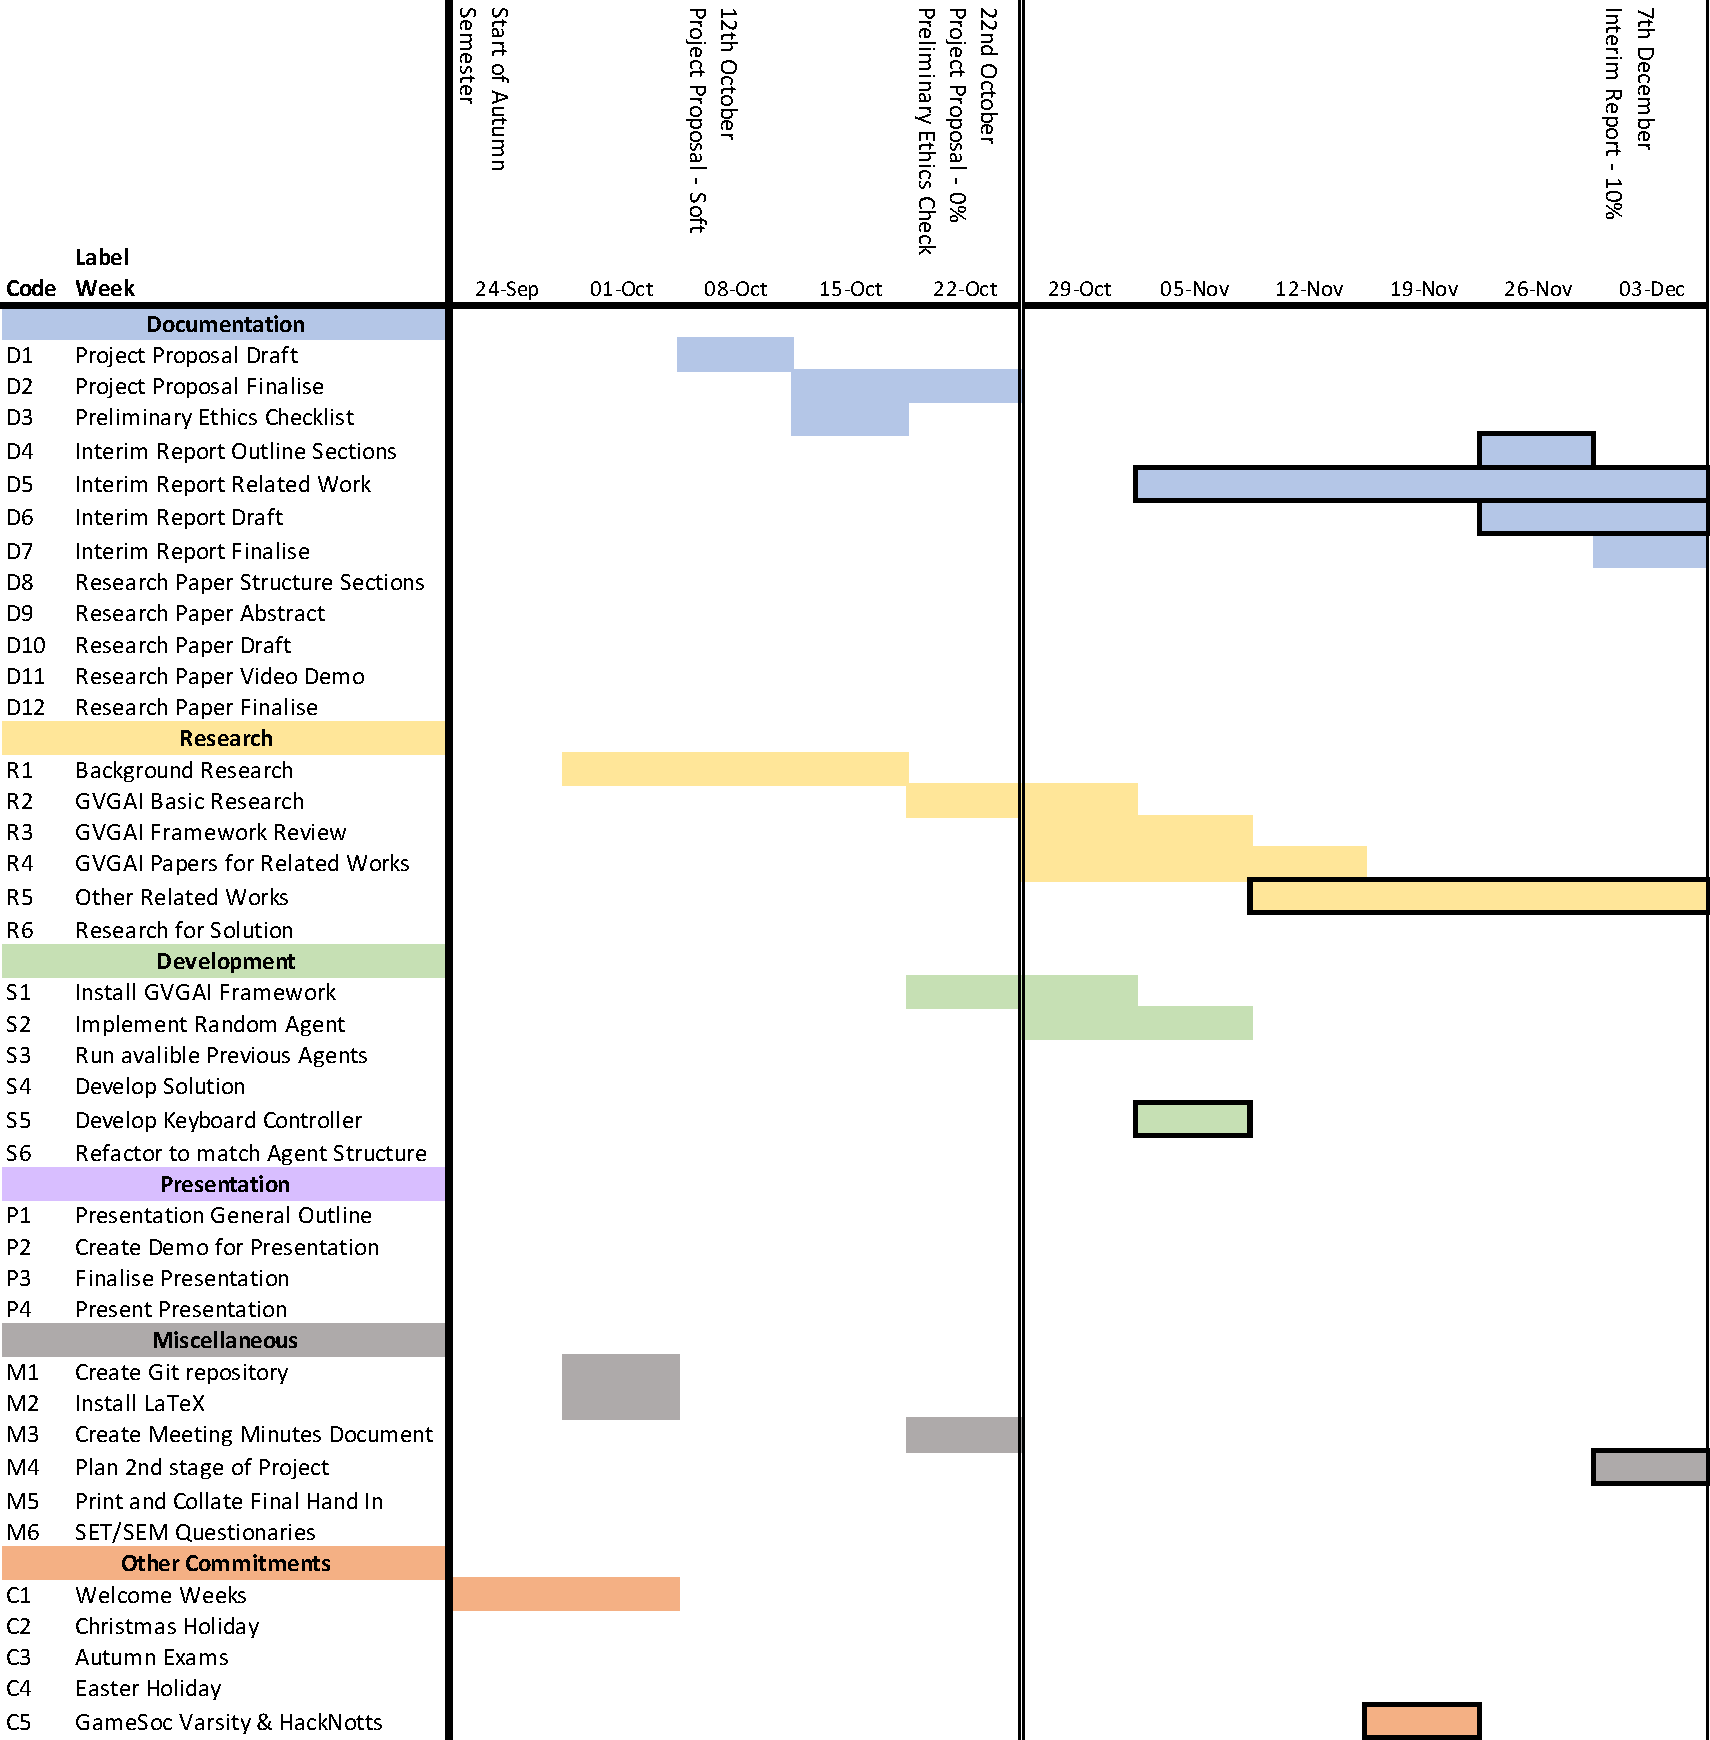
\includegraphics[width=17cm]{workPlan-7Dec.pdf} %17cm is 21cm of A4 width - (2cm * 2) margins
\end{center}
\subsubsection{7\textsuperscript{th} September --- 17\textsuperscript{th} May}
\begin{center}
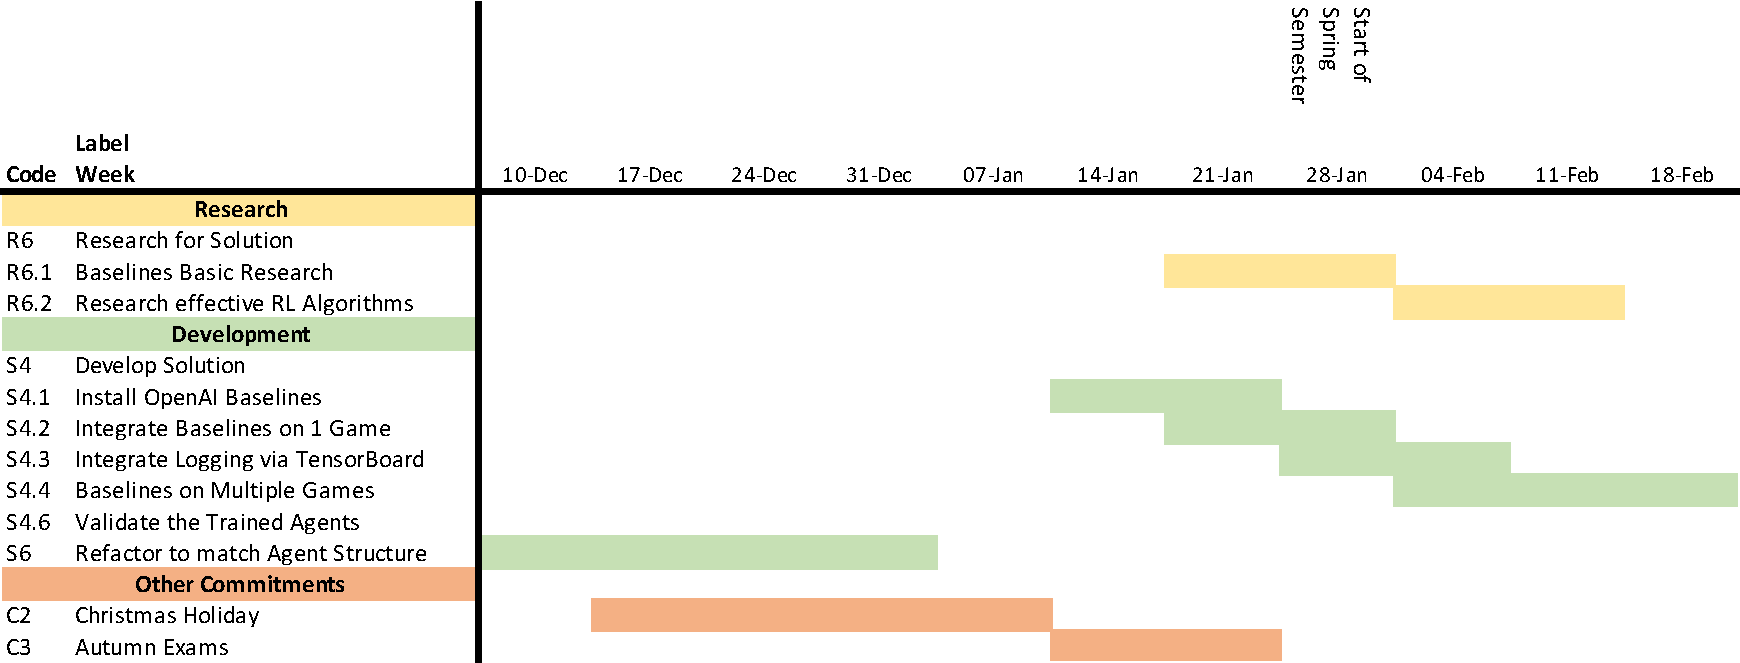
\includegraphics[width=17cm]{workPlan-18Feb.pdf} %17cm is 21cm of A4 width - (2cm * 2) margins
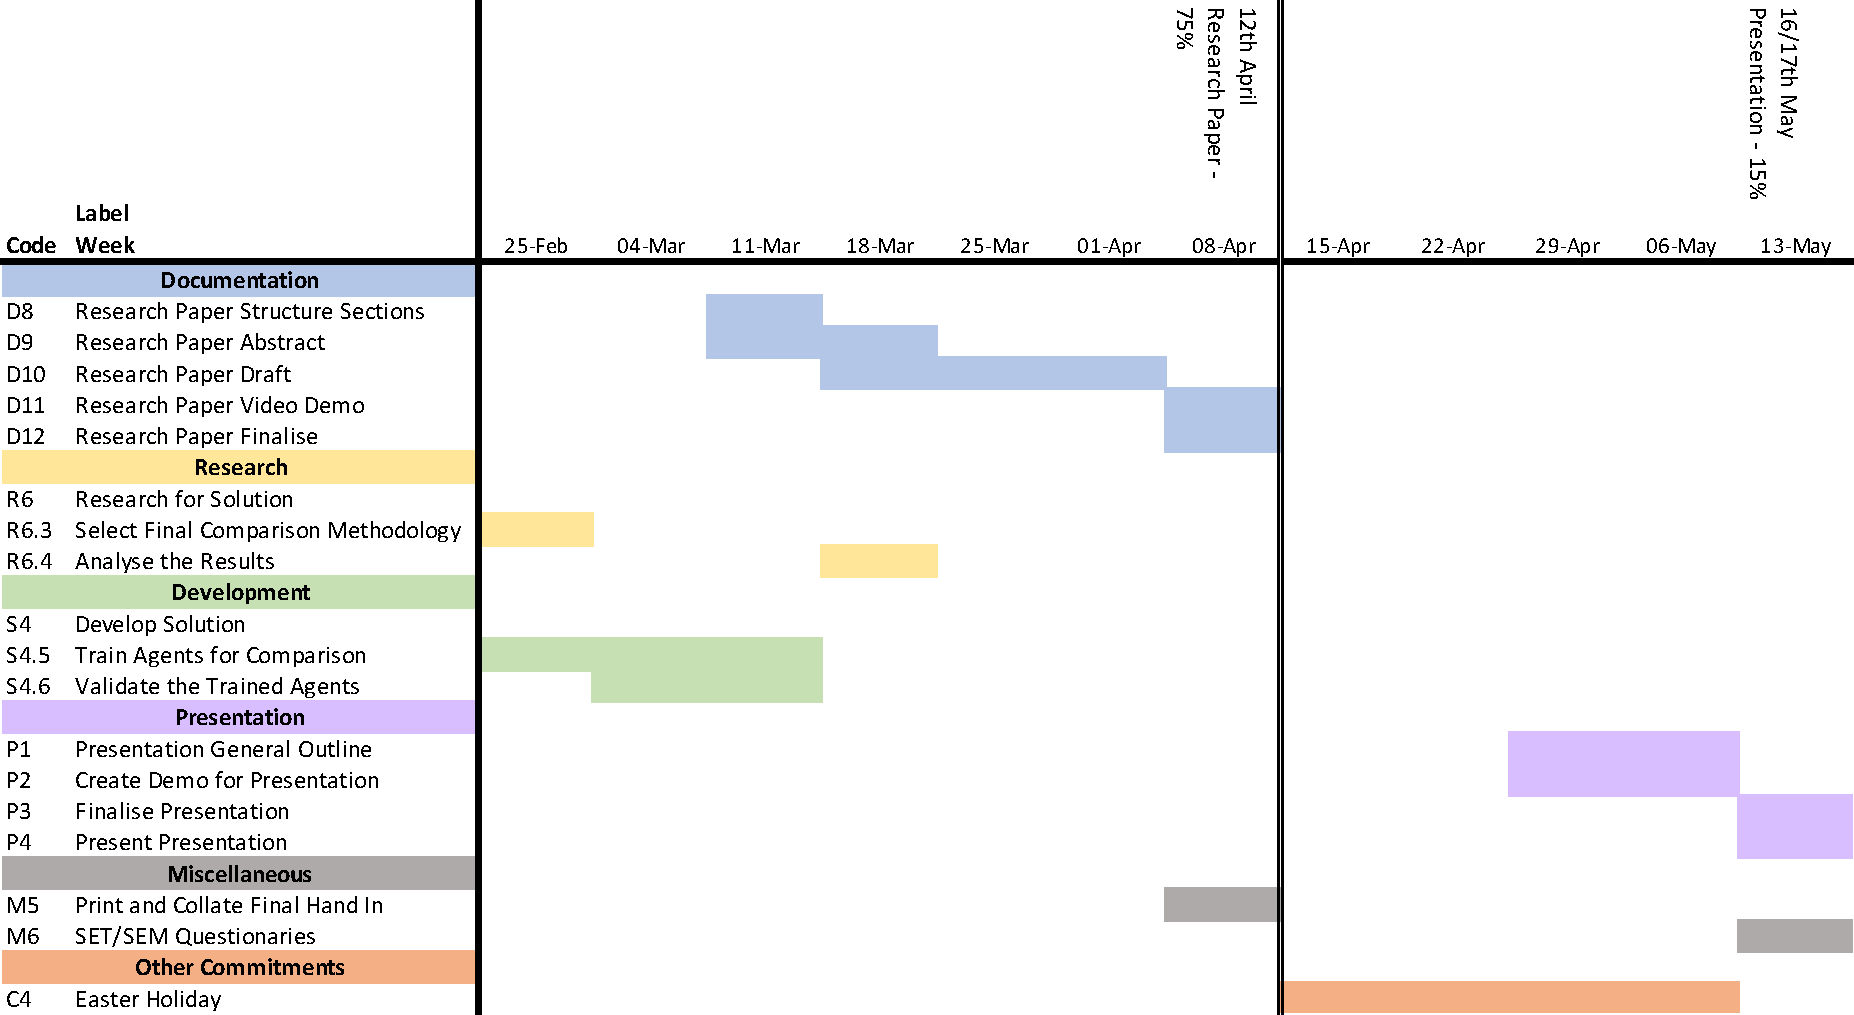
\includegraphics[width=17cm]{workPlan-17May.pdf} %17cm is 21cm of A4 width - (2cm * 2) margins

\end{center}


\end{document}
